\documentclass[10pt,letterpaper]{article}

\usepackage{cogsci}
\usepackage{pslatex}
\usepackage{apacite}
\usepackage{graphicx}
\usepackage{cleveref}
\usepackage{amsthm}
\usepackage{amsfonts}
\usepackage{amsmath}
\usepackage{algorithm}
\usepackage[]{algpseudocode}
\usepackage[labelfont=bf]{caption}
\usepackage[labelfont=bf]{subcaption}

\newtheorem{definition}{Definition}
\usepackage{pb-diagram,lamsarrow,pb-lams}

\usepackage[authormarkuptext=name,addedmarkup=bf,authormarkupposition=left]{changes}
%\usepackage[final]{changes} %Use this to hide all comments.
\definechangesauthor[name={D.~K.}, color={blue}]{dk}
\definechangesauthor[name={R.~W.}, color={red}]{rw}
\definechangesauthor[name={B.~L.}, color={green}]{bl}

\newcommand{\dkXX}[1]{\added[id=dk,remark={}]{#1}}
\newcommand{\rwXX}[1]{\added[id=rw,remark={}]{#1}}
\newcommand{\blXX}[1]{\added[id=bl,remark={}]{#1}}

\newcommand{\jsec}[1]{\marginpar{\fcolorbox{yellow}{yellow}{\parbox{0.7in}{\raggedright
        \color{blue} \tiny #1 }}}}
\newcommand{\hsec}[1]{\marginpar{\fcolorbox{yellow}{yellow}{\parbox{0.7in}{\raggedright
        \color{green} \tiny #1 }}}}
\newcommand{\jhmargin}[2]{{\color{orange}#1}\marginpar{\color{orange}\tiny\raggedright
    \bf [JH] #2}}



\title{On the Comparison of Pedestrian Intent Estimation by Humans and Machines}
 
\author{{\large \bf Dong-Ki Kim (dkkim93@mit.edu)} \\
  Laboratory for Information and Decision Systems 
  \AND {\large \bf Rose E. Wang (rewang@mit.edu)} \\
  Department of Electrical Engineering and Computer Science
  \AND {\large \bf Bj\"orn L\"utjens (lutjens@mit.edu)} \\
  Laboratory for Information and Decision Systems}

\begin{document}
\maketitle

\begin{abstract}
Human drivers excel in predicting the behavior of pedestrians on the sidewalk. The drivers observe pedestrian position, gaze, body pose and more to infer hidden variables that guide the future pedestrian trajectory. These hidden variables can be the pedestrian's goal, dynamics model and more. Autonomous vehicles need to copy the human capability to predict pedestrian intent to achieve to drive as safe and confident as humans. This project learns a Hidden Markov Model (HMM) and a neural network model to imitate human capabilities in estimating pedestrian intent. Especially for the neural network model, we experiment with two variants: one without uncertainty and another with uncertainty. Our results show, that the HMM resembles human decision making, by focusing on predictive euclidean distance, but misses out on unmodeled more complicated hidden states. In comparison to the HMM, the neural network model is more data hungry and better learned the underlying pedestrian behavior. Interestingly, the neural network with uncertainty estimate correlates with the human uncertainty.
\end{abstract}

%!TEX root=main.tex

\section{Introduction} \label{sec:intro}
For autonomous vehicles to drive fast and safe, it is important for the vehicles to correctly predict the intent (i.e., path prediction) of pedestrians, bicyclists, and drivers around them (\cref{fig:overview}). 
Previous works have attempted to predict intent of pedestrians and drivers. They have showed promising directions toward correctly estimating human intent, but the problem of correctly predicting the intent still remains challenging~\cite{Alahi2016, Morris2011}. 
On the other hand, humans excel at the task to estimate pedestrian and driver intent~\cite{Keller2014}. 
They exploit their intuitive understanding of physics~\cite{Battaglia2013} and hidden variables that describe human intent. Hidden variables can be the pedestrian's hidden goal, level of distraction, repulsiveness and attraction to other pedestrians or many more~\cite{Helbing1998}. Humans can infer these parameters for example from observing the body pose, gaze direction, mimic and observation of obstacles in the environment.

This project aims to understand human intent with computational models, such as the hidden Markov model (HMM) and a neural network model. The pedestrian prediction task is simplified as collision prediction task to allow for comparison.

First, a human is tasked to predict if two pedestrians are going to collide, given a simulated video sequence. Second, an HMM is learned to infer collision probability from the same data and the prior is adapted to better imitate the human predictive capabilities. Third, an ensemble of neural network is trained on a bigger dataset and it's predictive mean and uncertainty is compared against the human decision making. 

This project analyses the capability of humans to predict pedestrian intent and evaluates an HMM and Neural Network model to copy this capability. The HMM's posterior is adapted to closely resemble human decision making and indicates that humans strongly rely on the heading and euclidean distance information to predict collisions. The neural network model was trained to predict collision probability. Additionally, we use an ensemble of neural networks to estimate uncertainty. The neural network model achieves the Pearson correlation of $0.69$ between a human data and model's prediction. As we show, the neural network model is less capable to perform than humans to predict novel behavior, but interestingly is uncertain for the same region as humans are.

All source code and results can be found at 
$https://github.com/dkkim93/9.66\_collision\_final\_project$.

\begin{figure}[t]
  \centering
  \includegraphics[width=\linewidth]{figures/motivaton.png}
  \caption{Pedestrian intent estimation~\cite{Kooij2018}. Humans are experts in estimating pedestrian intent, i.e. predicting whether the pedestrian is going to cross (red) or not (green). 
  Using computational models, our objective is to understand the underlying mechanism behind human decision making for pedestrian intent estimation.}
  \label{fig:overview}
\end{figure}
%!TEX root=main.tex

\section{Related Work} \label{sec:related_work}

\subsection{Uncertainty in Neural Networks}
Neural networks have achieved state-of-the-art results on estimating human intent~\cite{Vemula2017, Alahi2016}. However, one fundamental difference in human and neural network reasoning is uncertainty. Neural networks normally predict a mean prediction value and can fail over-confidently on novel data. Humans, in comparison, would reveal their uncertainty saying \textit{I have never seen this behavior before, hence I do not know how to predict the behavior}. To give the neural networks a similar notion of uncertainty and \textit{know what they don't know}, we have explored the recent field uncertainty-aware neural networks. 

Bayesian Neural Networks reason about predictive uncertainty by keeping track of a distribution for each network's parameter~\cite{MacKay1992, Neal1996}. However, they are computationally intractable due to the expensive calculation of the Bayesian posterior. Even approximate methods, such as Markov Chain Monte Carlo or variational methods, come with extensive computational cost~\cite{Louizos2016, Graves2011, Springenberg_2016}. Other works, proposes MC-Dropout~\cite{Gal2015}: the activation of Dropout~\cite{Dropout2014} during test as approximate Bayesian inference in deep Gaussian processes. However, uncertainty estimates with MC-Dropout have shown to be overconfident on novel data~\cite{Osband2016, Lakshmi2016}. 

Alternative works proposes the Bootstrapping as an approximation of model uncertainty in neural networks~\cite{Osband2016, Lakshmi2016}. Intuitively, an ensemble of randomly initialized models is trained on overlapping samples of a training dataset and during test the sample variance of predictions indicates the ensemble uncertainty. The predictions of each model will be similar for data points that have often occurred in the training set and differ for data points that have only occurred in one sample of the training set or not occurred at all. 

\subsection{Intuitive physics understanding}
This work was inspired by \cite{Lerer, Bramley2017} who explored how to simulate our intuition about physics, and did so using deep feed-forward models to learn intuitive physics.

\begin{figure}[]
	\begin{subfigure}[]{1\linewidth}
		\centering
		\includegraphics[width=0.95\linewidth]{figures/sim_no_coll.png}
		\caption{Example trajectory with no collision.}
		\label{fig:sim_no_coll}
	\end{subfigure}
	\\
	\begin{subfigure}[]{1\linewidth}
		\centering
		\includegraphics[width=0.95\linewidth]{figures/sim_coll.png}
		\caption{Example trajectory with collision.}
		\label{fig:sim_coll}
	\end{subfigure}
    \caption{Pedestrian Simulation. In the beginning of each episode, the pedestrian simulation randomly spawns two pedestrians (dark orange and blue circle) at time $t=0$ at a random $x-y$ position. The simulation uses a pedestrian dynamics model to propagate the positions over time. The  bird's eye perspective of the pedestrian positions is displayed. At each time step the updated pedestrian position is plotted whose color becomes lighter over time. In ~\cref{fig:sim_no_coll} two pedestrians avoid each other and in~\cref{fig:sim_coll} two pedestrians collide.} 
    \label{fig:ped_sim}
\end{figure}

%!TEX root=main.tex

\section{Approach}\label{sec:approach}

\subsection{Generation of Pedestrian Trajectories in Simulation}
To compare the capability of humans and machines to predict pedestrian behavior, we have created a simulation of pedestrian behavior. For fairness, the simulation was designed to display the same information to human participants and the models.~\Cref{fig:ped_sim} shows multiple frames of pedestrian trajectories from the bird's eye view.

The simulation implements a dynamics model of pedestrians. Two pedestrians (orange and blue dot) are spawned with a random $x-y$ position and heading angle. The simulation assumes constant velocity $1m/s$, which is a common choice in pedestrian simulations~\cite{Sean2014}. The velocity is used to propagate the position of both agents over time with step size $0.2s$. The positions of both pedestrians are propagated over a maximum of 20 steps until an episode ends. The simulation records a collision label, when the distance of both pedestrians is smaller than the sum of their radius (circumference of the orange and blue circle). 

The simulation uses Reciprocal-Velocity-Obstacles (RVO2)~\cite{Vandenberg2008} as pedestrian dynamics model. Intuitively, each RVO2 pedestrian observes the other pedestrian's position and assumes that they will continue with their current heading and velocity forever. Based on this prediction, the RVO2 pedestrian chooses it's future path the way, that it is as close as possible to its' preferred path, but will never collide with the other agent. Because RVO2 guarantees that no pedestrians will collide, if they all follow RVO2, we have eliminated the possibility for the RVO2 pedestrians to adapt their velocity. This caused approximately 25\% collisions among all episodes.

Reciprocal Velocity Obstacles (RVO2)~\cite{Vandenberg2008} is a decentralized collision avoidance policy and has also been used in other works as pedestrian simulator~\cite{Bera2017}. In comparison to the social forces model~\cite{Helbing1998}, we have decided for the decentralized model RVO2. Decentralized, in this case, means that each pedestrian cannot directly observe the other pedestrian hidden states. We believe in the model being more realistic, because humans also decide about their future trajectory in a decentralized manner. 

RVO2 provides a collaboration coefficient $\alpha$ with determines how "aggressive" or "stubborn" a pedestrian behaves, i.e. it determines how much the pedestrian goes out of the way of the other pedestrian. In this works the parameter is set to the default $0.5$, but future works infers this parameter from real pedestrian data via Bayesian Inference, as demonstrated in~\cite{Bera2017}.

Two datasets have been generated. The first contains $89$ episodes with two pedestrians x-y position and heading over time. The dataset is used for the collection of intent estimation by humans and the HMM. The second dataset contains $8.5$k episodes without pictures and is used by the neural network model.

\begin{figure}[t]
  \centering
  \includegraphics[width=\linewidth]{figures/screenshot.png}
  \caption{A screenshot of human data collection. Each frame shows the trajectories of the two agents by the color gradient (where the lighter color implies the most recent). 
  After participants see a sequence of $5$ frames, they predict pedestrian intent. They do so by entering a rating from $0$ to $10$ which indicates their confidence in the prediction that the two pedestrians are going to collide.}
  \label{fig:human-data-collection}
\end{figure}

\subsection{Collection of Intent Estimation by Humans}
We have asked our participants the following question: \textit{``Assume two normal pedestrians. Normal as in they are ``partially'' cooperative and social pedestrians. Look at the following sequence of $5$ image frames that display two pedestrians' positions over time from the bird's eye view.
Now, how confident are you that the pedestrians' will collide in the near future ($15$ image frames)? Rate from $0$ to $10$ that describe your estimation ($0$: certainly no collision, $10$: certainly collision)''}. 
Our purpose of the question is to give a prior to our participants such that the two pedestrians in the simulator tend to avoid each other but not always (as the word ``partially'' implies). 

\Cref{fig:human-data-collection} shows a screenshot of a simple graphical user interface (GUI) that we have used to collect human data.
Each frame shows the two agents' trajectory, so participants do not need to go back or remember where robots were in the past frames. 
After our participants see the first five frames, they enter their rating from $0$ to $10$, where their responses are saved. 
With this procedure, we collected total $89$ human data samples from three individuals from scientific background. During simulation 24 of these samples have led to a collision, which induces a data set bias towards predicting no collision.
% \\
\\
\subsubsection{Analysis on Collected Human Data} 
\Cref{fig:histogram-human-data} shows the histogram of the ratings.
Interestingly, the histogram shows a bias towards the no collision ratings (i.e., rating $0$).
This might not only be caused by the dataset bias, but also by the question that participants read. 
Because the question mentions about the cooperative and social behaviors of pedestrians, people would have thought that two pedestrians are likely to avoid each other. The histogram reflects this biased prior. 
The data also shows two local maxima at scores $0-3$ and $4-8$ indicating that humans are more confident in prediction no collision than they are in predicting a collision. A possible explanation for this trend is the following: No collision ratings are very confident if the two pedestrians move in opposite directions, as seen in~\cref{fig:sim_no_coll}. When two pedestrians move in the direction of each other as seen in~\cref{fig:sim_coll}, the human prediction is less clear. 
\begin{figure}[t]
  \centering
  \includegraphics[width=\linewidth]{figures/human_hist.png}
  \caption{Histogram of Participants Ratings. 
  The histogram plots the frequency of the humans' predicted collision probability scores $[0,9]$ on $89$ samples. The histogram shows two peaks towards the no collision rating and a score around $6$. The biased question prior and the dataset bias could partly explain the bias towards the no collision rating. The simulation's ambiguity in a collision case as seen in~\cref{fig:sim_coll}, could explain lack of confidence in a human prediction towards collisions.}
  \label{fig:histogram-human-data}
\end{figure}

\subsection{Neural Network}\label{sec:neural-network}
A neural network (NN) model provides a stronger representation power with lots of learning parameters. 
A neural network model is also trained with a train dataset, which the model learns from and learns how to solve a task. 
One might connect the learning of a neural network model with a train dataset with a human learning from his/her previous experiences. 
Motivated by model's computational power and connection with human's prior experiences, we train a neural network (\cref{fig:nn-without-bootstrap}). We evaluate and analysis the model to understand better about human's decision making in the pedestrian intent prediction task.

Although the neural network model predicts a collision probability, it does not output about uncertainty in its prediction.
Uncertainty provides useful information such that we could use to understand what data points that the model is confused. It also provides a new perspective in understanding relationships between the neural network model and human (e.g., whether the model is also confused at what humans are unsure about). 
Therefore, we take a further step in the neural network model and measure the uncertainty in its prediction (\cref{fig:nn-with-bootstrap}). 
The uncertainty is measured via bootstrapping~\cite{Osband2016, Lakshmi2016}. 
Intuitively, an ensemble of randomly initialized models is trained on overlapping samples of a training dataset. 
Then, during the testing phase, the sample variance of predictions indicates the uncertainty in the prediction. 

\begin{figure}[t]
	\begin{subfigure}[t]{1\linewidth}
		\centering
		\includegraphics[width=0.95\linewidth]{figures/nn.pdf}
		\caption{Neural Network Model without Bootstrapping.}
		\label{fig:nn-without-bootstrap}
	\end{subfigure}
    \\
    \par\bigskip
	\begin{subfigure}[t]{1\linewidth}
		\centering
		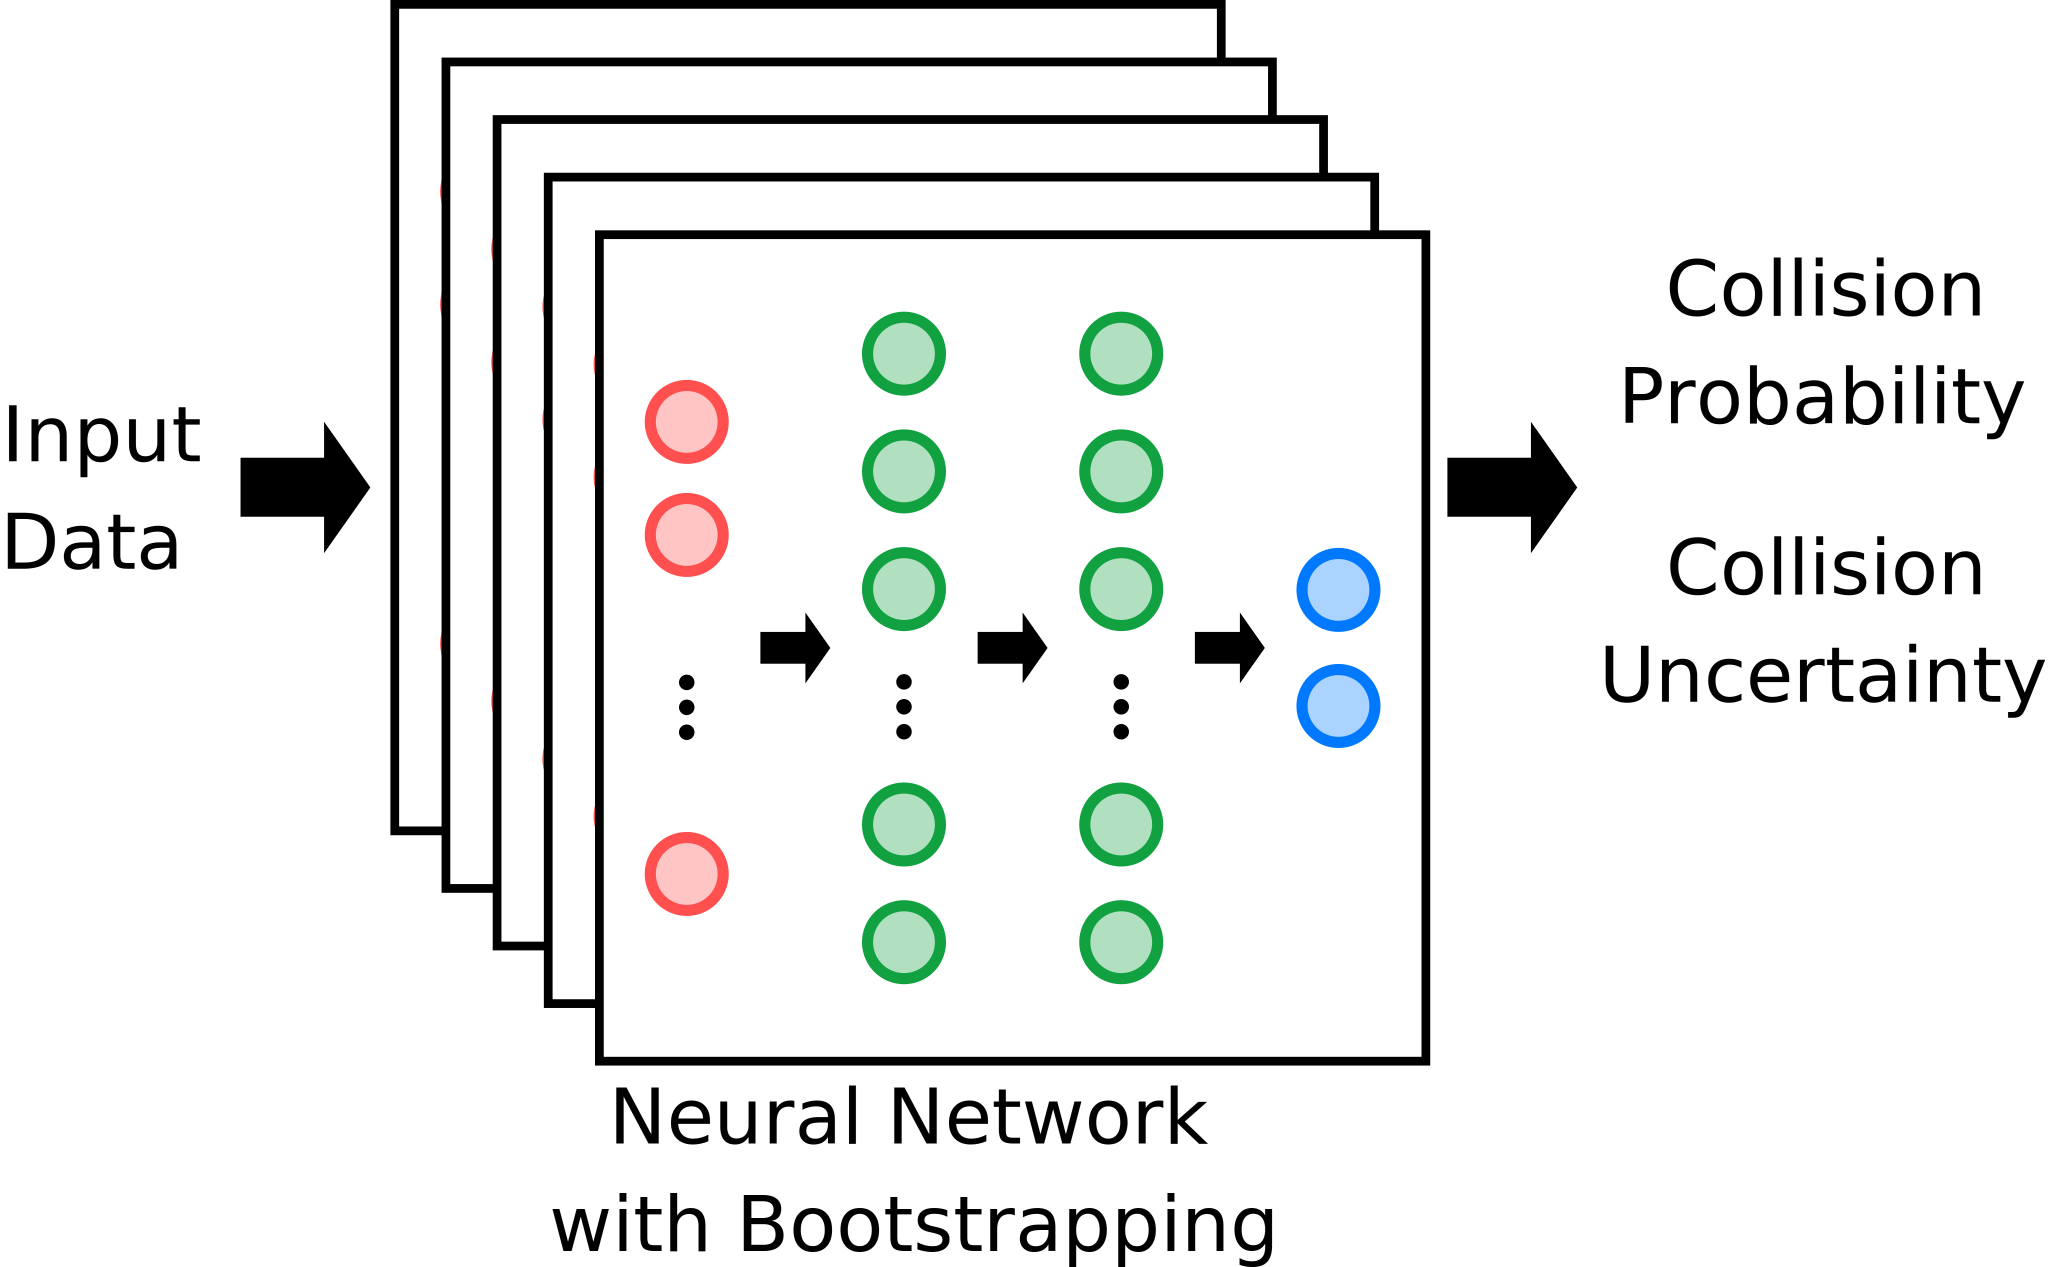
\includegraphics[width=0.95\linewidth]{figures/nn_bootstrap.pdf}
		\caption{Neural Network Model with Bootstrapping.}
		\label{fig:nn-with-bootstrap}
	\end{subfigure}
	\caption{Our two approaches for neural networks. (a) Neural network model with one feed-forward network. (b) Neural network model with Bootstrapping (i.e., ensemble of neural networks) for uncertainty. In (b) the collision probability and uncertainty is the sample mean and variance from the neural network ensemble's predictions.}
	\label{fig:nn-overview}
\end{figure}

\begin{algorithm}[t]
	\caption{Collision Neural Network}
	\label{alg:nn-without-bootstrapping}
	\begin{algorithmic}[1]
	    \Require Train, validation, and test dataset $\mathcal{D}_{train}$, $\mathcal{D}_{val}$, $\mathcal{D}_{test}$
	    \State Initialize a feed-forward neural network model $\mathcal{M}$
	    \State Train the network with train $\mathcal{D}_{train}$ and validation dataset $\mathcal{D}_{val}$
	    \State Test the network with test dataset $\mathcal{D}_{test}$ and get collision probabilities
	\end{algorithmic}
\end{algorithm}

\begin{algorithm}[t]
	\caption{Uncertainty-Aware Collision Neural Network Collision Model}
	\label{alg:nn-with-bootstrapping}
	\begin{algorithmic}[1]
	    \Require Train, validation, and test dataset $\mathcal{D}_{train}$, $\mathcal{D}_{val}$, $\mathcal{D}_{test}$
	    \Require Number of Bootstrapping $N$
	    \State Initialize feed-forward neural network models $\{\mathcal{M}_{1}, \mathcal{M}_{2}, ..., \mathcal{M}_{N} \}$
	    \For{each network $\mathcal{M}_{i}$}
	        \State Randomly shuffle train $\mathcal{D}_{train}$ and validation dataset $\mathcal{D}_{val}$
	        \State Train network $\mathcal{M}_{i}$ 
	    \EndFor
	    \For{each network $\mathcal{M}_{i}$}
	        \State Test network $\mathcal{M}_{i}$ with test dataset $\mathcal{D}_{test}$ and get collision probabilities
	    \EndFor
	    \State Get uncertainty by measuring sample variance in the collision probabilities of $N$ models
	\end{algorithmic}
\end{algorithm}

\begin{figure}[t]
  \centering
  \includegraphics[width=\linewidth]{figures/loss.png}
  \caption{Validation losses for training the neural network with bootstrapping. The validation loss decreases with variances, as desired.}
  \label{fig:ensemble-loss}
\end{figure}

\subsection{Network and Train Details}
Our neural network model is three-layer feed-forward deep neural network, consisting of rectified linear unit (ReLU) activation and $64$ nodes per layer.
A final layer of the softmax activation is used at the output of the policy that provides the collision probability. 
Because our participants only see the locations of two agents, we also provide only location information to the networks. 
Similar to \cite{mnih2015humanlevel}, where they concatenated multiple frames to avoid using a recurrent neural network, we concatenate location information across the first five frames and provide as an input to the network.
Please note that we could also consider using a convolutional neural network to effectively process with image data. 
However, the usage of convolutional layers would cause additional, unnecessary complexities both in learning and understanding between a human and neural network model, which motivated us to experiment based on a feed-forward network.

The (deep) neural networks require lots of data points for learning. 
Thus, from the pedestrian behavior simulation, we collected a sufficient amount of data: $8.5$k trajectories. 
Because collecting human participants' responses on all these data points are expensive, we consider a ground-truth of collision if a collision actually happened during these trajectories.
We divided the dataset with train and validation dataset\footnote{$20$\% of dataset is used as the validation dataset} and trained the neural network models (i.e., neural network model with and without bootstrapping). 
The ensemble size of $5$ is used for the neural network model with bootstrapping. 
The Adam optimizer with a learning rate of $0.0003$ is used. 
The validation data is used to decide to prevent the overfitting. 
\Cref{fig:ensemble-loss} shows the validation losses for the neural network model with bootstrapping. 
The losses are similar but with variances, as desired. 
Pseudocode for neural network model without and with bootstrapping are summarized in \cref{alg:nn-without-bootstrapping} and \cref{alg:nn-with-bootstrapping}, respectively. 

\subsection{Hidden Markov Model}
As black-box neural network alternative, we have implemented a fully introspective Hidden Markov Model (HMM). We thereby make the Markov assumption, i.e. \textit{the future is independent of the past, given the present}. In this case, the future pedestrian intent is independent of previous observations, given the current heading and position observation, and the model. The model's inference of pedestrian intent is converted into a collision prediction and compared and adapted to the humans' predictions. 

\begin{definition}
Formally, a hidden markov model is composed of the following.
\begin{itemize}
    \item a finite set of states $Q = \{q_1, ...,q_n\}$
    \item a transition matrix $A$, such that element $A_{i,j}$ describes the probability of transitioning from state $q_i$ to state $q_j$. 
    \item a finite set of observations $O = \{o_1,...,o_n\}$
    \item an output transition matrix $B$, such that $B_{i,j}$ describes the probability of observation $o_i$ being produced from state $q_j$
    \item an initial probability distribution $\Pi_n$ over the hidden states
\end{itemize}
\end{definition}

\subsection{Hidden Markov Model}
We consider the following structure for formulating collision prediction with a Hidden Markov Model. \\
The simulated data discussed in the prior section gives us information on the position, the speeds, and the orientation of the agent in global space. The underlying stochastic process that is not observable to outsiders is the intention of the agents. The intention of the agents is important in then determining how close they are willing to get, and, thus, the likelihood of collision. \\
Our fundamental problem setup for the HMM was: Given the observation sequence $O_1, O_2,...,O_T$, estimate the optimal sequence of hidden states. \\
Humans only have access to the sequence of relative positions and infer heading and velocity from the short video sequence. Similarly, the HMM only has access to the sequence of relative positions and does not access information about velocity. For model simplicity and a slight advantage, the HMM also accesses the sequence of pedestrian heading angles (i.e. where the pedestrian is looking).
\begin{enumerate}
    \item We place a Gaussian prior on the initially hidden intent. The internal states are discretized action possibilities in the $8$ directions depicted in \label{dir}: north, north-east, east, south-east, south, south-west, west, and north-west.
    \begin{figure}
        \centering
        \includegraphics[scale=0.5]{figures/compass.jpg}
        \caption{Considered 8 orientation directions for HMM: north, north-east, east, south-east, south, south-west, west, and north-west.}
        \label{fig:dir}
    \end{figure} \\ 
    \textbf{Note:} Similar to inferring, if a coin is loaded, one could adapt this prior to better match human knowledge. However, this mostly makes sense in domains, where the human has a strong prior about future direction, i.e. in a one-way street. As in our domain all directions can be seen equally likely, we have concentrated on adapting different parameters.
    \item The models are fitted to the first five time steps of observation data from each agent. We then want a sequence of optimal states for future agent actions. 
    The criterion we use to choose the states, $i$, is the state with most likelihood. To implement this solution, we let $\gamma$ be the probability of being in state $q_i$ at time $t+1$, given the observation sequence $O$ and the model $\lambda$.
    $$\gamma_{t+1}(i) = Pr(i_t=q_i|O, \lambda)$$
    We sample the model for the most likely state for the agent's orientation. In other words, 
    $$i_{t+1} = argmax[ \gamma_{t+1}(i)]$$
    \item Given the most likely state for the agent's orientation and the agent's last known position, we can predict the next positions of those agents. 
    \item We use both position models to derive a euclidean distance model between the agents. We calculate the euclidean distance from the position samples in the prior step. We create a euclidean distance model based on the euclidean distances. We define the discrete states of the distance model to range from $[0, 9]$. These are in the original graph units. 
    \item We use the euclidean distance model to then sample for the most likely euclidean distances. Collisions are defined based on a reasonable threshold distance $x$, where if the euclidean distance $d_t$ at time step $t$ is $d_t < x$, we determine there will be a collision. 
\end{enumerate}

%!TEX root=main.tex

\section{Results} \label{sec:results}
In this section, we explain our results with HMM and NN model.

\begin{figure}[t]
  \centering
  \includegraphics[width=\linewidth]{figures/nn_result.png}
  \caption{Comparisons between human responses and neural network model prediction. The Pearson correlation between the two data is $0.69$, which indicates a good linear relationship between neural network model and human decision making.}
  \label{fig:nn_raw_result}
\end{figure}

\begin{figure}[t]
	\begin{subfigure}[t]{1\linewidth}
		\centering
		\includegraphics[width=0.95\linewidth]{figures/agree.pdf}
		\caption{Agreed Test Data Points}
		\label{fig:nn-agree}
	\end{subfigure}
    \\
    \par\bigskip
	\begin{subfigure}[t]{1\linewidth}
		\centering
		\includegraphics[width=0.95\linewidth]{figures/disagree.pdf}
		\caption{Disagreed Test Data Points}
		\label{fig:nn-disagree}
	\end{subfigure}
	\caption{(a) Test data points that both human and neural network model predict to be zero collision. (b) Test data points that human and the model strongly disagree. Left: $P_{collision} = 0.3$ (human response) vs $1.0$ (neural network prediction probability). Center: $0.7$ vs $0.1$. Right: $0.7$ vs $0.0$.}
	\label{fig:nn-analysis}
\end{figure}

\begin{figure}[t]
  \centering
  \includegraphics[width=\linewidth]{figures/nn_hist.png}
  \caption{Histogram of neural network prediction on the test dataset. Similar to the human responses, the result shows a bias toward no-collision. The neural network model is more confident than the human in its' collision predictions.}
  \label{fig:nn_hist}
\end{figure}

\subsection{Neural Network}
We consider two neural network models: one without bootstrapping and the other with bootstrapping. 
Compared to the model without bootstrapping, the model with bootstrapping provides additional information about uncertainty.
In this section, we first demonstrate our result with neural network without bootstrapping and then discuss further analysis with uncertainty.

\begin{figure}[t]
  \centering
  \includegraphics[width=\linewidth]{figures/uncertainty.png}
  \caption{Uncertainty of the neural network predictions on the test dataset. Peaks mostly correspond to ambiguous situations as depicted in~\cref{fig:nn-uncertain-data}, which displays datapoint $27$.}
  \label{fig:nn-uncertainty}
\end{figure}

\begin{figure}[t]
  \centering
  \includegraphics[width=\linewidth]{figures/unceratin_data.png}
  \caption{Test data point with id $27$ that both neural network and human are confused about. The neural network indicates confusion by the standard deviation (i.e., uncertainty) of $0.11$. The test participants have rated  $0.6$ collision probability, which is close to a random guess ($0.5$).}
  \label{fig:nn-uncertain-data}
\end{figure}

\begin{figure}[t]
  \centering
  \includegraphics[width=\linewidth]{figures/noise_data.png}
  \caption{The test data with Gaussian noise. Gaussian noise has never been observed in the neural network's training dataset. On the novel observation with Gaussian noise (wiggly trajectory), the neural networks' predictions are more likely to be erroneous. The uncertainty-aware model can identify these novel scenarios and similar to the human \textit{know what it does not know}.}
  \label{fig:noise-data}
\end{figure}

% \begin{figure}[t]
% 	\begin{subfigure}[t]{1\linewidth}
% 		\centering
% 		\includegraphics[width=0.95\linewidth]{figures/hmm_agree.pdf}
% 		\caption{Agreed Test Data Points for HMM}
% 		\label{fig:hmm-agree}
% 	\end{subfigure}
%     \\
%     \par\bigskip
% 	\begin{subfigure}[t]{1\linewidth}
% 		\centering
% 		\includegraphics[width=0.95\linewidth]{figures/hmm_disagree.pdf}
% 		\caption{Disagreed Test Data Points for HMM}
% 		\label{fig:hmm-disagree}
% 	\end{subfigure}
% 	\caption{(a) Test data points that both human and HMM predict to be no collision. (b) Test data points that human and HMM strongly disagree. Left: $P_{collision}=0.7$ (human response) vs no-collision (HMM prediction). Right: $0.7$ vs no-collision.}
% 	\label{fig:hmm-agree-disagree}
% \end{figure}

\subsubsection{Neural Network without Bootstrapping}
We first trained the network with the aforementioned training procedure.
Then we \textit{tested} the trained model using the data used to collect human responses\footnote{We hereafter refer the data used to collect human responses as \textit{test} dataset.}.

The comparison between the (normalized) human ratings and predicted collision probabilities by the neural network model is shown in \cref{fig:nn_raw_result}.
The Pearson correlation between the two data is $0.69$\footnote{A correlation of 0 means no linear relationship. A correlation of 1 or -1 means a strong positive linear or negative relationship.}, which shows a good linear relationship between the two. Motivated by their linear relationship, we generate the histogram of the neural network model's prediction to see whether it also shows a bias toward the no-collision similar to human responses (see \cref{fig:human-data-collection}).
\Cref{fig:nn_hist} shows the histogram of the neural network prediction on the test dataset. Similar to the human responses, it does show a bias toward the no-collision. 
However, compared to the human responses, it has a much stronger bias toward the no collision probability. 

We delve deeper into the neural network model analysis by looking at test data points that human and the model strongly agree or disagree.
\cref{fig:nn-agree} shows test data points that both human and neural network model predicts the same collision probability of zero. 
These data points commonly show a trend that the two agents are heading to very different directions each other with sufficiently far distances. 
It is plausible for both humans and neural network model that the trend is a good reason to decide why the agents are not likely to collide.
On the other hand, \cref{fig:nn-disagree} describes another test data points that human and the model predict opposite decision (e.g., human predicts to be likely no collision but neural network model predicts to be collision).
Based on these test data points, humans are likely to predict collision if the two agents are close. However, if the two agents tend to move in a same direction, then human tends to give no collision.
However, the neural network model seems to be more sensitive to the orientation instead of the distance.% So if bad why is it? what can be done better?
\\

\subsubsection{Neural Network with Bootstrapping}
Uncertainty about NN model's prediction provides useful information such that we could use to understand what data points that the model is confused at. 
The uncertainty in its prediction is measured by the bootstrapping~\cite{Osband2016, Lakshmi2016}. 
The uncertainty about collision probability on test data points is shown in \cref{fig:nn-uncertainty}. Also, \cref{fig:nn-uncertain-data} shows the test data point that the NN model is the most confused at.
The model predicted a collision probability of $0.76$ with a standard deviation of $0.11$. 
It is understandable as a small orientation change could cause either collision or no collision.
This is also an interesting result because a human would be also confused at the same data point. Thus, we have adapted the neural network model to have a closer decision making to humans, compared to the neural network model without uncertainty.

\subsubsection{Neural Network Model with a Novel Data Point}
When a human is experienced with a new problem, he or she would have a little confident in solving the problem.  
Would the same capability exist in the neural network model? 
Would the uncertainty estimate provide the neural network model to be similar to a human?
To answer our questions, we generated a new data that significantly differs from our train dataset. 
Compared to the train dataset, which is noise-free, the new data has a large noise in its heading: for each time, we added a Gaussian noise with a mean of $0$ degree and a standard deviation of $30$ degree to each agent's heading.
The data is shown in \cref{fig:noise-data}. Interestingly, the neural network model with uncertainity predicted a collision probability of $0.69$ and a standard deviation (i.e., uncertainty) of $0.28$. 
Considering that the most biggest standard deviation in the test dataset was $0.11$ (see \cref{fig:nn-uncertainty}), the uncertainty on the new data is large. 
This result is desirable as we would expect the network to output a large uncertainty because the data significantly differs to the ones in the train dataset.
Considering a human would be also uncertain about a new situation that he or she never has experienced before, this result conveys that the neural network with uncertainty resembles better a human decision making compared to the model without uncertainty.

\subsection{Hidden Markov Model}
% \subsubsection{Limitations of the H
The HMM is able to model the closeness between agents to a limited degree.

Although it captures the notion of "small" and "large" distances given the orientations and positions of the agents, it is unable to model increasing and decreasing distances without any additional observations. It lacks the richness of human experiences to "forward" its physics engine. The model also doesn't understand agent intention: it lacks an intuitive psychology model and assumes that agent will continue going in the same direction. \\
Furthermore, the solution is implemented using the most likely orientation state. The implementation does not consider the global structure of observations, the neighboring states (with respect to timing), and the length of the observations. This type of "instantaneous optimality" can be problematic as it does not capture the overall sequential structure of the problem. \\
Nevertheless, the HMM allows for easy adaptation to the collected human data. By simply varying the prior $Pr(d) = i \forall d \in [0,9]$, where $d$ is the euclidean distance between the two agents are we able to have some intuition behind how human reason about collision physics and intention.~\Cref{fig:hmm-coll-pred} shows that the uniform prior on state probabilities matches the actual count of collisions across the $89$ experiments. Changing the prior to favor fewer collisions allows the frequency counts of the HMM to be more similar to the human results. \\
From this comparison, we can make a general conclusion that humans are more likely to predict collisions, when the observed distance in between the pedestrians in low. Intuitively, this makes sense. Additionally, the HMM was able to imitate the bias humans have towards predicting no collision and a small second bias in a collision score between $5-7$.

\begin{figure}[t]
	\begin{subfigure}[t]{1\linewidth}
		\centering
		\includegraphics[width=0.95\linewidth]{figures/hmm_prior.png}
		\caption{Before posterior update.}
		\label{fig:hmm-coll-pred-prior}
	\end{subfigure}
	\begin{subfigure}[t]{1\linewidth}
		\centering
		\includegraphics[width=0.95\linewidth]{figures/hmm_posterior.png}
		\caption{After posterior update.}
		\label{fig:hmm-coll-pred-post}
	\end{subfigure}
	\caption{HMM collision prediction. The HMM predicts a collision rating on the scale from $0$ to $9$ for $89$ sample trajectories. The HMM inference with default parameters in~\cref{fig:hmm-coll-pred-prior} deviates strongly from the human prediction in~\cref{fig:histogram-human-data}. We then adapt the parameters in~\cref{fig:hmm-coll-pred-post} to imitate human decision making. Similar to the human prediction, the HMM after posterior update has a bias towards "no collision" and has a low second peak around collision likelihood $5-7$.}
	\label{fig:hmm-coll-pred}
\end{figure}
\\

% This leads to an interesting discussion of where the collisions are being identified in each experiment. \dkXX{Insert graphics similar to fig 9 here.}.

% \iffalse
% \begin{figure}[t]
% 	\begin{subfigure}[t]{1\linewidth}
% 		\centering
% 		\includegraphics[scale=0.50]{figures/hmm_e_0.png}
% 		\caption{Sampling the distance HMM in experiment 0.}
% 		\label{fig:nn}
% 	\end{subfigure}
%     \\
%     \par\bigskip
% 	\begin{subfigure}[t]{1\linewidth}
% 		\centering
% 		\includegraphics[scale=0.25]{figures/course_966_e_00_t_05.png}
% 		\caption{The five timesteps of information given to the HMM.}
% 		\label{fig:nn-bootstrap}
% 	\end{subfigure}
% 	\caption{Experiment 0: HMM results against the observations. In this scenario, it looks like the two agents are very close to colliding: given their heading information, it seems like their paths will intersect.}
% 	\label{fig:nn-overview}
% \end{figure}

% \begin{figure}[t]
% 	\begin{subfigure}[t]{1\linewidth}
% 		\centering
% 		\includegraphics[scale=0.50]{figures/hmm_e_5.png}
% 		\caption{Sampling the distance HMM in experiment 0.}
% 		\label{fig:nn}
% 	\end{subfigure}
%     \\
%     \par\bigskip
% 	\begin{subfigure}[t]{1\linewidth}
% 		\centering
% 		\includegraphics[scale=0.25]{figures/course_966_e_05_t_05.png}
% 		\caption{The five timesteps of information given to the HMM.}
% 		\label{fig:nn-bootstrap}
% 	\end{subfigure}
% 	\caption{HMM results against the observations. }
% 	\label{fig:nn-overview}
% \end{figure}

% \begin{figure}[t]
% 	\begin{subfigure}[t]{1\linewidth}
% 		\centering
% 		\includegraphics[scale=0.50]{figures/hmm_e_8.png}
% 		\caption{Sampling the distance HMM in experiment 0.}
% 		\label{fig:nn}
% 	\end{subfigure}
%     \\
%     \par\bigskip
% 	\begin{subfigure}[t]{1\linewidth}
% 		\centering
% 		\includegraphics[scale=0.25]{figures/course_966_e_08_t_05.png}
% 		\caption{The five timesteps of information given to the HMM.}
% 		\label{fig:nn-bootstrap}
% 	\end{subfigure}
% 	\caption{HMM results against the observations.}
% 	\label{fig:nn-overview}
% \end{figure}

% \begin{figure}[t]
% 	\begin{subfigure}[t]{1\linewidth}
% 		\centering
% 		\includegraphics[scale=0.50]{figures/hmm_e_12.png}
% 		\caption{Sampling the distance HMM in experiment 0.}
% 		\label{fig:nn}
% 	\end{subfigure}
%     \\
%     \par\bigskip
% 	\begin{subfigure}[t]{1\linewidth}
% 		\centering
% 		\includegraphics[scale=0.25]{figures/course_966_e_12_t_05.png}
% 		\caption{The five timesteps of information given to the HMM.}
% 		\label{fig:nn-bootstrap}
% 	\end{subfigure}
% 	\caption{HMM results against the observations.}
% 	\label{fig:nn-overview}
% \end{figure}

% \begin{figure}[t]
% 	\begin{subfigure}[t]{1\linewidth}
% 		\centering
% 		\includegraphics[scale=0.50]{figures/hmm_e_14.png}
% 		\caption{Sampling the distance HMM in experiment 0.}
% 		\label{fig:nn}
% 	\end{subfigure}
%     \\
%     \par\bigskip
% 	\begin{subfigure}[t]{1\linewidth}
% 		\centering
% 		\includegraphics[scale=0.25]{figures/course_966_e_14_t_05.png}
% 		\caption{The five timesteps of information given to the HMM.}
% 		\label{fig:nn-bootstrap}
% 	\end{subfigure}
% 	\caption{HMM results against the observations.}
% 	\label{fig:nn-overview}
% \end{figure}
% \fi
%!TEX root=main.tex

\section{Conclusion} \label{sec:conclusion}
We have developed model that aimed to understand human capabilities in the task of pedestrian intent estimation. The analysis of a neural network and HMM shows that humans strongly rely on euclidean distance and inferred pedestrian heading to predict a possible collision in between two pedestrians. We have augmented a classic neural network to reason about its' predictive uncertainty. In comparison to a classic model, the uncertainty-aware model more closely resembles human prediction, because it is able to \textit{know what it doesn't know}.

\section{Work Division} \label{sec:work-division}
The tasks were split evenly and all decisions and analyses were taken jointly. 
% Bj\"orn has focused on the implementation of the pedestrian simulation, Rose on the implementation of HMM and Dong-Ki on the neural network implementation.

\section{Acknowledgments}

We appreciate Professor Joshua Tenenbaum's guidance and 9.660 TAs' insightful feedback on our project.

\newpage
\bibliographystyle{apacite}
\setlength{\bibleftmargin}{.125in}
\setlength{\bibindent}{-\bibleftmargin}
\bibliography{references}

\end{document}